\documentclass[11pt,oneside]{article}
\input{../../../Header/packages.sty}
\input{../../../Header/mathexpressions.sty}
\usepackage{fancyhdr}
\pagestyle{fancy}
\fancyhf{}
\lhead{Lektionsplanung: Die Flächenformel nach Heron}
\rhead{Jonas Guler (Gu)}
\rfoot{\thepage}
\renewcommand{\headrulewidth}{0.4pt}
\setlength{\headheight}{14pt}
\setlength{\parindent}{0pt}
\setlength{\parskip}{4pt}
\linespread{1.15}

\begin{document}
{\Large\textbf{Lektionsplanung: Die Flächenformel nach Heron}}\\[2mm]
\begin{tabularx}{\textwidth}{@{}lX}
	Thema: & Satzgruppe des Pythagoras, Abschluss: Flächeninhalt eines beliebigen Dreiecks aus drei Seiten\\
	Dauer: & 1 Lektion à 45 Minuten\\
	Einbettung: & nach Pythagoras, Kathetensatz und Höhensatz (Skript \textit{Sätze im rechtwinkligen Dreieck}, Abschnitt 3; dort ist der Abschnitt \textit{Die Flächenformel nach Heron} noch leer)\\
	Material: & Arbeitsblatt \texttt{heron.pdf}, Taschenrechner\\
\end{tabularx}

\section*{Lernziele}
Die Lernenden \ldots
\begin{itemize}[itemsep=0pt]
	\item berechnen in einem nicht rechtwinkligen Dreieck aus den drei Seiten mit zweimal Pythagoras die Höhe und den Flächeninhalt.
	\item leiten die Formel $A^2=s(s-a)(s-b)(s-c)$ selbst her, indem sie den Zahlenweg mit Variablen wiederholen (zweimal Pythagoras, zweimal 3.\ binomische Formel).
	\item kennen die Formel von Heron, wissen, dass sie für jedes Dreieck gilt, und können die Herleitung in ihren vier Schritten wiedergeben.
	\item berechnen mit der Formel Flächeninhalte und Höhen, auch in Anwendungen (Vierecke über eine Diagonale zerlegen), und erkennen an der Formel, wann ein Dreieck nicht existiert.
\end{itemize}

\textbf{Vorwissen:} Satz des Pythagoras, Höhe im gleichseitigen Dreieck, binomische Formeln, Kongruenzsatz SSS, Dreiecksungleichung (implizit).

\textbf{Kernbotschaft:} Drei Seiten legen ein Dreieck und damit seinen Flächeninhalt fest. Heron berechnet ihn direkt, und die Formel ist nichts anderes als \textit{zweimal Pythagoras plus Algebra}.

\section*{Ablauf}
\renewcommand{\arraystretch}{1.3}
\begin{tabularx}{\textwidth}{|>{\raggedright\arraybackslash}p{11mm}|>{\raggedright\arraybackslash}p{27mm}|X|>{\raggedright\arraybackslash}p{22mm}|}\hline
	\textbf{Zeit} & \textbf{Phase} & \textbf{Inhalt und Aktivität} & \textbf{Sozialform}\\\hline
	0'--3' & Einstieg & Begrüssung. Impulsfrage: \textit{Ein Dreieck mit den Seiten 13, 14, 15 cm. Wie gross ist seine Fläche? Was fehlt uns?} (Antwort: eine Höhe.) Lektionsziel: \textit{Fläche nur aus den Seiten.} Arbeitsblatt austeilen. & Plenum\\\hline
	3'--18' & Schüleraktivität (Repetition + Herleitung) & \textbf{Aufgabe 1.1, Teil A} (ca.\ 5'): zweimal Pythagoras, $x=5$, $h_c=12$, $A=84$. \textbf{Teil B} (ca.\ 10'): derselbe Weg mit $a,b,c$ als geführter Lückentext: Pythagoras $\to x$, $h_c^2=(b+x)(b-x)$, zweimal 3.\ binomische Formel, $A^2=\frac{1}{16}(a+b+c)\cdots$, dann halber Umfang $s$ einführen. Kontrolle mit 13/14/15 und 3/4/5. Nach ca.\ 8' bei Bedarf Zwischenhalt im Plenum zu e)/f). & Partnerarbeit\\\hline
	18'--25' & Theorieinput & Ergebnisse aus h) sammeln. \textbf{Satz 2.1} an die Wandtafel, Heron kurz historisch einordnen. \textbf{Beweis} als Zusammenfassung der vier Schritte aus Teil B (Lehrperson zeigt die Rechnung zu f)--h) vollständig, falls Paare nicht fertig wurden). \textbf{Bemerkungen:} Symmetrie, Rechenschema mit Kontrolle $(s-a)+(s-b)+(s-c)=s$, Höhen aus $h_a=\frac{2A}{a}$. \textbf{Beispiel 1} gemeinsam (ca.\ 3'). & Plenum, Lehrervortrag mit Fragen\\\hline
	25'--44' & Übungen & \textbf{Pflicht:} Aufgabe 3.1 a)--d), 3.2, 3.3.\newline \textbf{Zusatz:} 3.1 e)--f), 3.4 (Grundstück), 3.5 (Formel streikt), 3.6 $\bigstar$ (Heron-Dreiecke), 3.7 $\bigstar$ (Inkreis). Lösungen liegen bei der Lehrperson auf bzw.\ werden ab Min.\ 38 aufgelegt. & Einzel- oder Partnerarbeit\\\hline
	44'--45' & Abschluss & Merksatz wiederholen lassen: \textit{Halber Umfang $s$, dann $\sqrt{s(s-a)(s-b)(s-c)}$.} Hausaufgabe: Pflichtaufgaben fertig, 3.5. & Plenum\\\hline
\end{tabularx}

\section*{Tafelbild (Vorschlag)}
\begin{minipage}{0.55\linewidth}
	\textbf{Flächenformel nach Heron}\\
	$s=\dfrac{a+b+c}{2}$ (halber Umfang)
	\[A=\sqrt{s\,(s-a)\,(s-b)\,(s-c)}\]
	\textbf{Beweisidee:} $h_c^2=b^2-x^2=a^2-(c-x)^2$ (2$\times$ Pythagoras)\\ $\Rightarrow x=\frac{b^2+c^2-a^2}{2c}$, $h_c^2=(b+x)(b-x)$\\ 3.\ binomische Formel $\Rightarrow A^2=\frac14c^2h_c^2=s(s-a)(s-b)(s-c)$.\\[1mm]
	\textbf{Beispiel:} $13,14,15$: $s=21$, $A=\sqrt{21\cdot8\cdot7\cdot6}=84$.
\end{minipage}
\hfill
\begin{minipage}{0.4\linewidth}
	\centering
	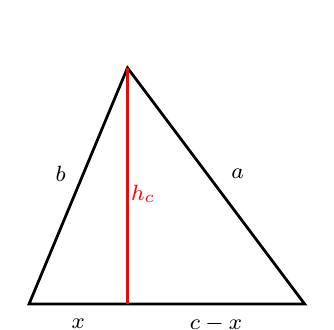
\begin{tikzpicture}[x=1cm, y=1cm, font=\footnotesize, scale=0.5]
		\draw[line width=1pt] (0,0) -- (7,0) -- (2.5,6) -- cycle;
		\draw[red, line width=1pt] (2.5,6) -- (2.5,0);
		\draw (1.25,-0.5) node {$x$};
		\draw (4.75,-0.5) node {$c-x$};
		\draw (0.8,3.3) node {$b$};
		\draw (5.3,3.3) node {$a$};
		\draw[red] (2.9,2.8) node {$h_c$};
	\end{tikzpicture}
\end{minipage}

\section*{Mögliche Schwierigkeiten und Differenzierung}
\begin{itemize}[itemsep=0pt]
	\item \textbf{Teil A der Einstiegsaufgabe:} Wer nicht weiterkommt, erhält den Hinweis \textit{Beide Teildreiecke haben die Höhe $h_c$ gemeinsam.} Klammer $(14-x)^2$ ist eine Fehlerquelle (binomische Formel).
	\item \textbf{Teil B (Algebra):} Die kritischen Stellen sind e) (auf einen Bruchstrich, $b^2+2bc+c^2$ als $(b+c)^2$ erkennen) und f) ($a^2-(b-c)^2$ zerlegen, Vorzeichen in $a-b+c$). Hilfsimpuls: \textit{Wo steht ein Quadrat minus ein Quadrat?} Bei Zeitnot e)--f) im Plenum gemeinsam, g)--i) wieder in Partnerarbeit.
	\item \textbf{Rechenfehler:} $s$ mit dem ganzen Umfang verwechseln; zu früh runden. Rechenschema an die Tafel und konsequent erst am Schluss die Wurzel ziehen.
	\item \textbf{Höhen:} Faktor 2 in $h_a=\frac{2A}{a}$ wird oft vergessen.
	\item \textbf{Schwächere Lernende:} Teil A mit dem Tipp \textit{$x=5$, kontrolliere!} abkürzen. In Teil B Hilfekarte mit den Zwischenresultaten von e) und f) bereithalten.
	\item \textbf{Stärkere Lernende:} Teil B ohne Lückentext auf einem leeren Blatt herleiten; 3.6 $\bigstar$ (Heron-Dreiecke) und 3.7 $\bigstar$ (Inkreis).
\end{itemize}

\newpage
\section*{Lösungen}
\textbf{Aufgabe 1.1}
\begin{itemize}[itemsep=0pt]
	\item[a)] $h_c^2=13^2-x^2$ und $h_c^2=15^2-(14-x)^2$.
	\item[b)] $169-x^2=225-196+28x-x^2\ \Rightarrow\ 140=28x\ \Rightarrow\ x=5$\,cm.
	\item[c)] $h_c=\sqrt{169-25}=12$\,cm, $A=\frac{14\cdot12}{2}=84$\,cm$^2$.
	\item[d)] $h_c^2=b^2-x^2$ und $h_c^2=a^2-(c-x)^2$. Gleichsetzen: $b^2-x^2=a^2-c^2+2cx-x^2\Rightarrow x=\frac{b^2+c^2-a^2}{2c}$.
	\item[e)] $b+x=\frac{(b+c)^2-a^2}{2c}$, $b-x=\frac{a^2-(b-c)^2}{2c}$.
	\item[f)] $(b+c)^2-a^2=(b+c+a)(b+c-a)$, $a^2-(b-c)^2=(a-b+c)(a+b-c)$.
	\item[g)] $A^2=\frac14c^2\cdot\frac{(a+b+c)(b+c-a)(a-b+c)(a+b-c)}{4c^2}=\frac{(a+b+c)(b+c-a)(a-b+c)(a+b-c)}{16}$.
	\item[h)] $b+c-a=a+b+c-2a=2s-2a=2(s-a)$, $a-b+c=2(s-b)$, $a+b-c=2(s-c)$. $A^2=\frac{2s\cdot2(s-a)\cdot2(s-b)\cdot2(s-c)}{16}=s(s-a)(s-b)(s-c)$, also $A=\sqrt{s(s-a)(s-b)(s-c)}$.
	\item[i)] $13,14,15$: $s=21$, $A=\sqrt{21\cdot8\cdot7\cdot6}=\sqrt{7056}=84$ (stimmt). $3,4,5$: $s=6$, $A=\sqrt{6\cdot3\cdot2\cdot1}=6=\frac{3\cdot4}{2}$ (stimmt).
\end{itemize}

\textbf{Beispiel 1:} $s=12$, $A=\sqrt{12\cdot5\cdot4\cdot3}=\sqrt{720}=12\sqrt5\approx26.83$\,cm$^2$, $h_c=\frac{2A}{9}=\frac{8\sqrt5}{3}\approx5.96$\,cm.

\textbf{Aufgabe 3.1}
\begin{enumerate}[label=\alph*), itemsep=0pt]
	\item $s=15$, $A=\sqrt{15\cdot10\cdot3\cdot2}=\sqrt{900}=30$\,cm$^2$. Kontrolle: $\frac{5\cdot12}{2}=30$.
	\item $s=16$, $A=\sqrt{16\cdot6\cdot6\cdot4}=\sqrt{2304}=48$\,cm$^2$. Kontrolle: Höhe auf die Basis $\sqrt{100-36}=8$, $\frac{12\cdot8}{2}=48$.
	\item $s=7.5$, $A=\sqrt{7.5\cdot3.5\cdot2.5\cdot1.5}=\sqrt{98.4375}=\frac{15}{4}\sqrt7\approx9.92$\,cm$^2$.
	\item $s=10.5$, $A=\sqrt{10.5\cdot4.5\cdot3.5\cdot2.5}=\sqrt{413.4375}=\frac{21}{4}\sqrt{15}\approx20.33$\,cm$^2$.
	\item $s=7.5$, $A=\sqrt{7.5\cdot5\cdot1.5\cdot1}=\sqrt{56.25}=7.5$\,cm$^2$. Kontrolle (rechtwinklig, $2.5^2+6^2=6.5^2$): $\frac{2.5\cdot6}{2}=7.5$.
	\item $s=18$, $A=\sqrt{18\cdot9\cdot8\cdot1}=\sqrt{1296}=36$\,cm$^2$ (stumpfwinkliges Dreieck, die Formel funktioniert trotzdem).
\end{enumerate}

\textbf{Aufgabe 3.2:} $s=60$, $A=\sqrt{60\cdot35\cdot21\cdot4}=\sqrt{176400}=420$\,cm$^2$. $h_a=\frac{840}{25}=33.6$\,cm, $h_b=\frac{840}{39}\approx21.54$\,cm, $h_c=\frac{840}{56}=15$\,cm. Die längste Höhe steht auf der kürzesten Seite, weil das Produkt Seite $\cdot$ Höhe immer $2A$ ergibt.

\textbf{Aufgabe 3.3:} $s=\frac{3a}{2}$, $s-a=s-b=s-c=\frac a2$. $A=\sqrt{\frac{3a}{2}\cdot\frac{a^3}{8}}=\sqrt{\frac{3a^4}{16}}=\frac{\sqrt3}{4}a^2$. Kontrolle: $\frac12\cdot a\cdot\frac a2\sqrt3=\frac{\sqrt3}{4}a^2$.

\textbf{Aufgabe 3.4:} $\triangle ABC$: $s=55$, $A_1=\sqrt{55\cdot15\cdot30\cdot10}=\sqrt{247500}\approx497.49$\,m$^2$. $\triangle ACD$: $s=55$, $A_2=\sqrt{55\cdot25\cdot20\cdot10}=\sqrt{275000}\approx524.40$\,m$^2$. Total $\approx1021.9$\,m$^2$, Preis $\approx868\,600$ Fr.

\textbf{Aufgabe 3.5:} a) $s=7$, $s-c=0$, also $A=0$: Wegen $3+4=7$ liegen die drei Punkte auf einer Geraden, das Dreieck ist ausgeartet. b) $s=5.5$, $s-c=-0.5$, unter der Wurzel steht $-24.0625<0$: Wegen $2+3<6$ lässt sich kein Dreieck konstruieren, die Kreisbögen schneiden sich nicht. Allgemein: Es braucht $s-a>0$, $s-b>0$, $s-c>0$, d.h.\ jede Seite ist kürzer als die Summe der beiden anderen (Dreiecksungleichung).

\textbf{Aufgabe 3.6:} a) $x=5$ und $h_c=12$: die Dreiecke $5,12,13$ und $9,12,15$, entlang der Kathete $12$ aneinandergelegt ($5+9=14$). b) Neues Dreieck $13,20,21$ (Basis $5+16=21$). Über die Teildreiecke: $\frac{5\cdot12}{2}+\frac{16\cdot12}{2}=30+96=126$. Heron: $s=27$, $A=\sqrt{27\cdot14\cdot7\cdot6}=\sqrt{15876}=126$ (stimmt). c) z.B.\ $5,5,8$ ($A=12$), $10,13,13$ ($A=60$), $25,39,56$ ($A=420$) oder durch Aneinanderlegen weiterer pythagoreischer Dreiecke mit gleicher Kathete.

\textbf{Aufgabe 3.7:} a) Die drei Teildreiecke haben die Grundseiten $a$, $b$, $c$ und alle die Höhe $r$ (Inkreis berührt die Seiten senkrecht zum Radius): $A=\frac12ar+\frac12br+\frac12cr=r\cdot s$. b) $r=\frac{A}{s}=\frac{84}{21}=4$.

\section*{Quellen und Inspiration}
\begin{itemize}[itemsep=0pt]
	\item Geometrie 1 Aufgaben (Niederberger), Kap.\,5 \textit{Die Satzgruppe im rechtwinkligen Dreieck}, S.\,88, Nr.\,81 (Überprüfen an pythagoreischen und gleichseitigen Dreiecken, geführte Herleitung in Teil d)): Ideen für 1.1 Teil B, 3.1 und 3.3.
	\item Skript \texttt{Skripts/Geometrie/2\_sätzedreieck}: Höhe im gleichseitigen Dreieck (Bezug in 3.3). Der Abschnitt \textit{Die Flächenformel nach Heron} ist dort noch leer; das Arbeitsblatt kann als Vorlage dafür dienen.
	\item Prüfungssammlung \texttt{SchoolTex/Exams} (Pools, Prüfungen, \_Archiv, GZP25, Trigonometrie, Vektorgeometrie) geprüft: Keine Aufgabe zur Formel von Heron, zu Heron-Dreiecken, zum Inkreisradius oder zur Dreiecksungleichung vorhanden. Alle Übungsaufgaben sind neu.
\end{itemize}
\end{document}
